\documentclass[tikz]{standalone}% 'crop' is the default for v1.0, before it was 'preview'
%\usetikzlibrary{...}% tikz package already loaded by 'tikz' option
\usepackage{subcaption}
\usepackage[compat=1.1.0]{tikz-feynman}

\begin{document}

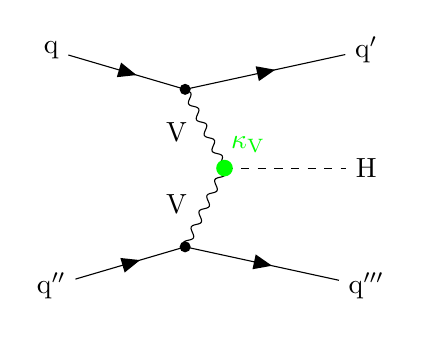
\begin{tikzpicture}
  
  \begin{feynman}
    \vertex at (0,3) (top) {$\mathrm{q}$};
    \vertex at (0,2.5) (midtop);
    \vertex at (0,1.5) (mid);
    \vertex at (0,0.5) (midbot);
    \vertex at (0,0) (bot) {$\mathrm{q}^{\prime\prime}$};
    \vertex at (1.7,2.5) (vtop);
    \vertex at (2.2,1.5) (kappa);
    \vertex at (1.7,0.5) (vbot);
    \vertex at (4.0,1.5) (h) {H};
    \vertex at (4.0,3) (finaltop) {$\mathrm{q}^{\prime}$};
    \vertex at (4.0,0) (finalbot) {$\mathrm{q}^{\prime\prime\prime}$};
    
    \diagram* [horizontal=mid to h] {
      (top) -- [fermion] (vtop) -- [fermion] (finaltop),
      (bot) -- [fermion] (vbot) -- [fermion] (finalbot),
      (vtop) -- [boson, edge label = $\mathrm{V}$, swap, pos=0.3] (kappa) -- [boson, edge label = $\mathrm{V}$, swap, pos=0.7] (vbot),
      (kappa) -- [scalar] (h),
    };
  \end{feynman}

  \fill[green] (kappa) circle (3pt);
  \node[green] at ($(kappa) + (0.3,0.3)$) {$\kappa_{\mathrm{V}}$};
  \fill[black] (vtop) circle (2pt);
  \fill[black] (vbot) circle (2pt);
  
\end{tikzpicture}

\end{document}
